
\subsection[{\ce{CO2}} flow with pressure dependent density and viscosity]{{\ce{CO2}} flow with pressure dependent density and viscosity (H-process)}

%\subsubsection{}
 
\subsubsection*{Problem definition}

This benchmark shows the distribution of pressure along a 1D soil profile for different fluid property models (see Fig.~\ref{fig-eos-probdef}). Two wells, one injection well and one production well are placed with a distance of $\unit[400]{m}$. $\mathrm{CO_2}$ is dumped by the injection well at a pressure of $\unit[7]{MPa}$, at the production well there is a pressure of $\unit[6.5]{MPa}$. The temperature along the profile shall be constant at $\unit[400]{K}$.  
 
 
\begin{figure}[h]
\centering
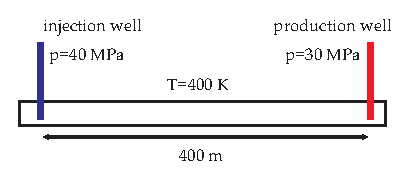
\includegraphics[width=0.5\textwidth]{FLUID_PROPERTIES/figures/Prob-def.eps}
\caption{Problem definition}
\label{fig-eos-probdef}
\end{figure}

\subsubsection*{Model setup}
For this case the model area is reduced to a very simple 1D problem. The mesh consists of 200 line elements with a constant length of $\unit[2]{m}$. The injection well on the left side is represented as a constant boundary pressure of $\unit[40]{MPa}$, the right boundary has a constant pressure of $\unit[30]{MPa}$ for the whole domain. Initial conditions are a temperature of $\unit[400]{K}$ and a pressure of $\unit[30]{MPa}$. The used material is a porous medium with a porosity of $\mathrm{n_e}=\unit[10]{\%}$ and a density of $\mathrm{\rho}=\unit[2500]{kg\,m^{-3}}$. 

\subsubsection*{Fluid properties}

Two different cases show the influence of non linear fluid properties. A constant viscosity of $\mathrm{\eta}=\unit[0.001]{Pa\,s}$ in the first simulation is set. For the second simulation, the \co2 viscosity is calculated by a constant temperature and a pressure depending density. The calculation is based on data tables with $\rho\hspace{0.04cm}p\hspace{0.04cm}T$-data calculated by \eqref{eq-fhe1} and on the data set of 
$\rho\hspace{0.04cm}p\hspace{0.04cm}T$-data shown in the appendix in Tabs.~\ref{appendix:co2_1} to \ref{appendix:co2_5}.

\subsubsection*{Results}

The pressure distribution for the first simulation with the constant visocosity decreases linearly along the profile. When viscosity and density are variable values the pressure distribution curve shows a non-linear behaviour like in Fig.~\ref{fig-eos-result}.

\begin{figure}[h]
\centering
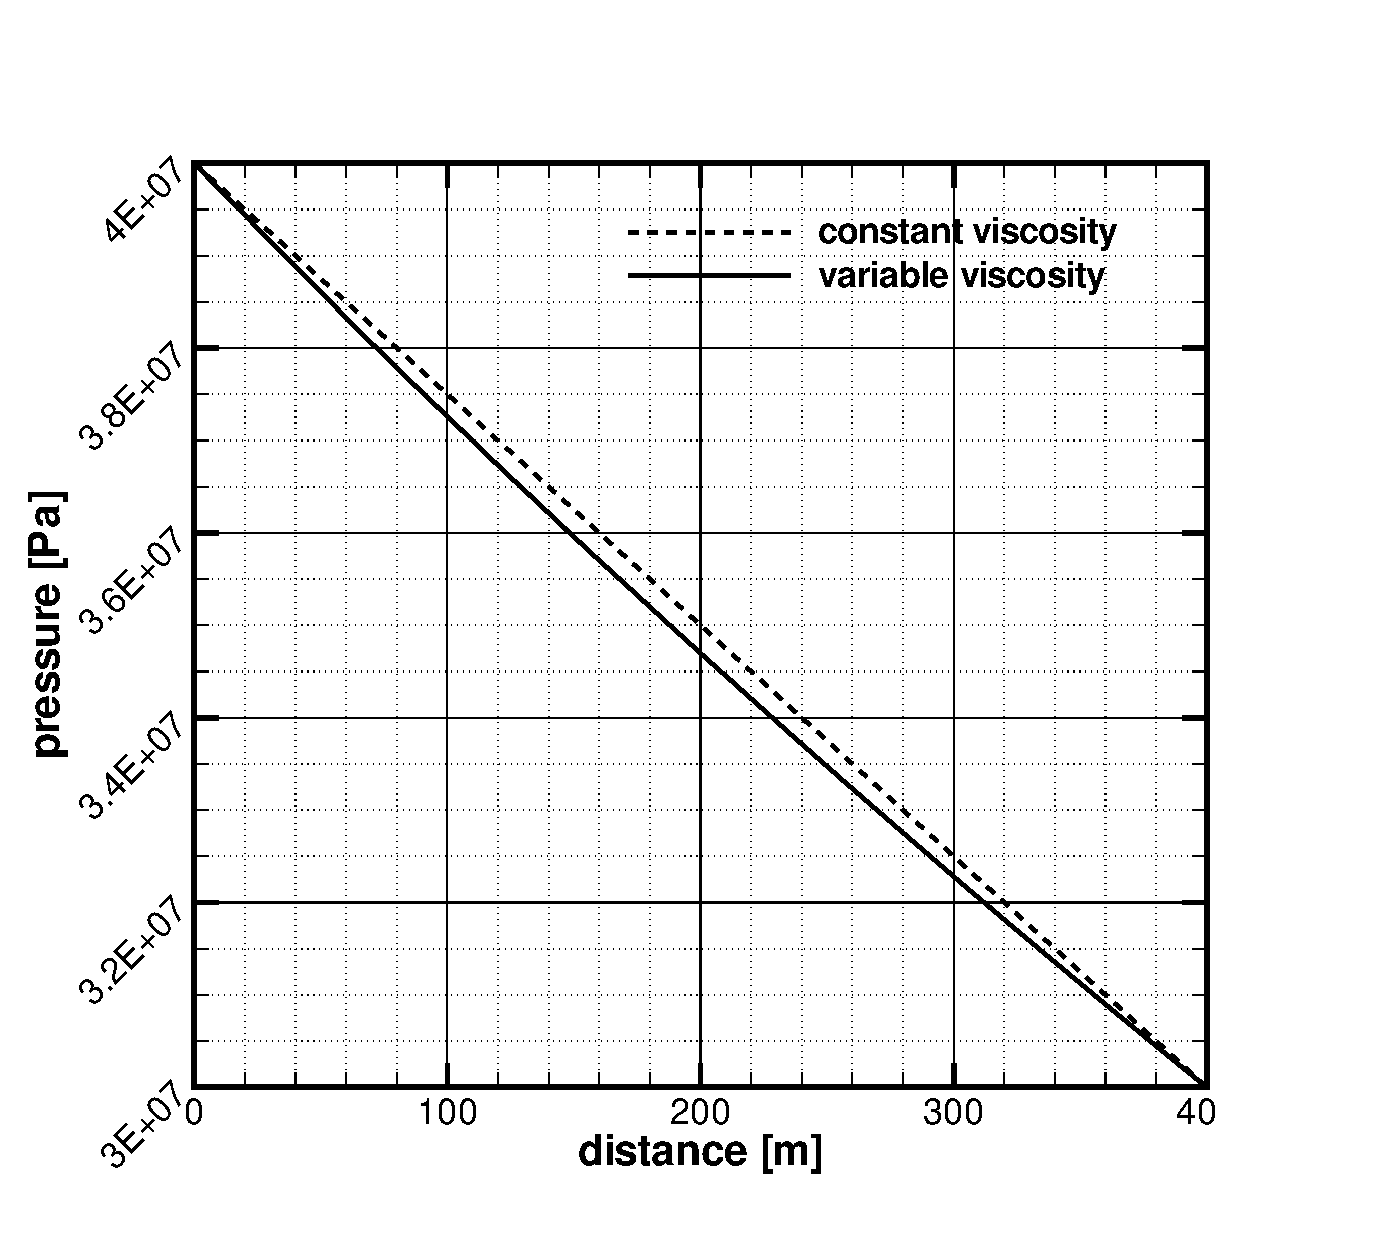
\includegraphics[width=0.8\textwidth]{FLUID_PROPERTIES/figures/result-co2-flow.eps}
\caption{\label{fig-eos-result}Pressure distribution along the soil profile}
\end{figure}
\subsubsection*{Benchmark deposit}
%
%\begin{tabular}{|l|l|l|}
%  \hline
%  Benchmark & Problem type & Path in benchmark deposit \\
%  \hline
%  CO2-FLOW & H & benchmarks\verb \GROUNDWATER_FLOW\CO2-FLOW \\
%  \hline
%\end{tabular}
%


\begin{table}[H]
  \caption[]{Benchmark location in the repository.}
 \begin{center}
 \begin{tabular}{lll}
  \toprule
  Benchmark & Problem type & Path in benchmark deposit \\
  \midrule
  CO2-FLOW & H & benchmarks\verb \GROUNDWATER_FLOW\CO2-FLOW \\
   \bottomrule
 \end{tabular}
 \end{center}
\end{table}
